\chapter{Optimization}


\section{Definitions}


\subsection{Unconstrained optimization}

\begin{description}
    \item[Unconstrained optimization] \marginnote{Unconstrained optimization}
        Problem of form:
        \[ \min_{\z \in \mathbb{R}^d} l(\z) \]
        where $l: \mathbb{R}^d \rightarrow \mathbb{R}$ is the cost function and $\z$ the decision variables.
\end{description}

\begin{theorem}[First-order necessary condition of optimality] \marginnote{First-order necessary condition of optimality}
    Given a point $\z^*$ and a cost function $l: \mathbb{R}^d \rightarrow \mathbb{R}$ such that $l \in C^1$ in $B(\z^*, \varepsilon)$ (i.e., neighbors of $\z^*$ within a radius $\varepsilon$), it holds that:
    \[
        \z^* \text{ is local minimum } \Rightarrow \nabla l(\z^*) = 0
    \]
\end{theorem}

\begin{theorem}[Second-order necessary condition of optimality] \marginnote{Second-order necessary condition of optimality}
    Given a point $\z^*$ and a cost function $l: \mathbb{R}^d \rightarrow \mathbb{R}$ such that $l \in C^2$ in $B(\z^*, \varepsilon)$, it holds that:
    \[
        \z^* \text{ is local minimum } \Rightarrow \nabla^2 l(\z^*) \geq 0 \text{ (i.e., positive semidefinite)}
    \]
\end{theorem}


\subsection{Convexity}

\begin{description}
    \item[Convex set] \marginnote{Convex set}
        A set $Z \subseteq \mathbb{R}^d$ is convex if it holds that:
        \[
            \forall \z_A, \z_B \in Z: \Big( \forall \alpha \in [0, 1]: (\alpha \z_A + (1-\alpha)\z_B) \in Z \Big)
        \]

        \begin{figure}[H]
            \centering
            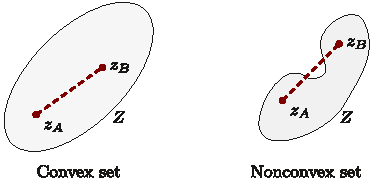
\includegraphics[width=0.4\linewidth]{img/_convex_set.pdf}
        \end{figure}

    \item[Convex function] \marginnote{Convex function}
        Given a convex set $Z \subseteq \mathbb{R}^d$, a function $l: Z \rightarrow \mathbb{R}$ is convex if it holds that:
        \[
            \forall \z_A, \z_B \in Z: \Big( \forall \alpha \in [0, 1]: l(\alpha \z_A + (1-\alpha) \z_B) \leq \alpha l(\z_A) + (1-\alpha) l(\z_B) \Big)
        \]

        \begin{figure}[H]
            \centering
            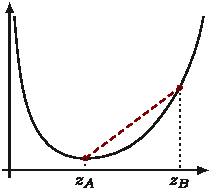
\includegraphics[width=0.25\linewidth]{img/_convex_function.pdf}
        \end{figure}

        \begin{remark}
            Given a differentiable and convex function $l: Z \rightarrow \mathbb{R}$, it holds that any of its points lie above all its tangents:
            \[ \forall \z_A, \z_B \in Z: l(\z_B) \geq l(\z_A) + \nabla l(\z_A)^T (\z_B - \z_A) \]

            \begin{figure}[H]
                \centering
                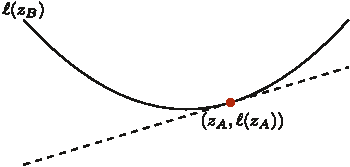
\includegraphics[width=0.3\linewidth]{img/_convex_tangent.pdf}
            \end{figure}
        \end{remark}

    \item[Strongly convex function] \marginnote{Strongly convex function}
        Given a convex set $Z \subseteq \mathbb{R}^d$, a function $l: Z \rightarrow \mathbb{R}$ is strongly convex with parameter $\mu > 0$ if it holds that:
        \[
            \begin{split}
                \forall \z_A, \z_B \in Z, \z_A \neq \z_B: \Big( \forall \alpha \in (0, 1)&: l(\alpha \z_A + (1-\alpha) \z_B) < \\
                &\alpha l(\z_A) + (1-\alpha) l(\z_B) - \frac{1}{2} \mu \alpha (1-\alpha) \Vert \z_A-\z_B \Vert^2 \Big)
            \end{split}
        \]
        Intuitively, it is strictly convex and grows as fast as a quadratic function.

        \begin{remark}
            Given a differentiable and $\mu$-strongly convex function $l: Z \rightarrow \mathbb{R}$, it holds that any of its points lie above all the paraboloids with curvature determined by $\mu$ and tangent to a point of the function:
            \[ \forall \z_A, \z_B \in Z: l(\z_B) \geq l(\z_A) + \nabla l(\z_A)^T (\z_B - \z_A) + \frac{\mu}{2} \Vert \z_B - \z_A \Vert^2 \]

            \begin{figure}[H]
                \centering
                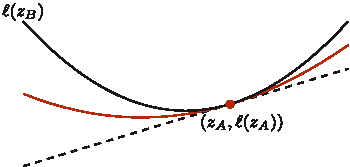
\includegraphics[width=0.35\linewidth]{img/_strongly_convex.pdf}
            \end{figure}

            A geometric interpretation is that strong convexity imposes a quadratic lower-bound to the function.
        \end{remark}
\end{description}

\begin{lemma}[Convexity and gradient monotonicity] \marginnote{Convexity and gradient monotonicity}
    Given a differentiable and convex function $l$, its gradient $\nabla l$ is a monotone operator, which means that it satisfies:
    \[
        \forall \z_A, \z_B: \big( \nabla l(\z_A) - \nabla l(\z_B) \big)^T (\z_A - \z_B) \geq 0
    \]
\end{lemma}

\begin{lemma}[Strict convexity and gradient monotonicity] \marginnote{Strict convexity and gradient monotonicity}
    Given a differentiable and strictly convex function $l$, its gradient $\nabla l$ is a strictly monotone operator, which means that it satisfies:
    \[
        \forall \z_A, \z_B: \big( \nabla l(\z_A) - \nabla l(\z_B) \big)^T (\z_A - \z_B) > 0
    \]
\end{lemma}

\begin{lemma}[Strong convexity and gradient monotonicity] \marginnote{Strong convexity and gradient monotonicity}
    Given a differentiable and $\mu$-strongly convex function $l$, its gradient $\nabla l$ is a strongly monotone operator, which means that it satisfies:
    \[
        \forall \z_A, \z_B: \big( \nabla l(\z_A) - \nabla l(\z_B) \big)^T (\z_A - \z_B) \geq \mu \Vert \z_A - \z_B \Vert^2
    \]
\end{lemma}

\begin{description}
    \item[Lipschitz continuity] \marginnote{Lipschitz continuity}
        Given a function $l$, it is Lipschitz continuous with parameter $L > 0$ if:
        \[
            \forall \z_A, \z_B: \Vert l(\z_A) - l(\z_B) \Vert \leq L \Vert \z_A - \z_B \Vert
        \]

        \begin{remark}
            Given a differentiable function $l$ with $L$-Lipschitz continuous gradient $\nabla l$, it holds that any of its points lie below all the paraboloids with curvature determined by $L$ and tangent to a point of the function:
            \[ \forall \z_A, \z_B \in Z: l(\z_B) \leq l(\z_A) + \nabla l(\z_A)^T (\z_B - \z_A) + \frac{L}{2} \Vert \z_B - \z_A \Vert^2 \]

            \begin{figure}[H]
                \centering
                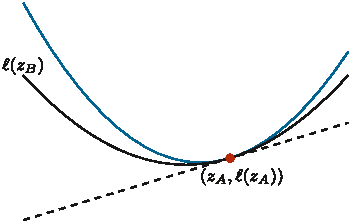
\includegraphics[width=0.35\linewidth]{img/_lipschitz_gradient.pdf}
            \end{figure}

            A geometric interpretation is that Lipschitz continuity of the gradient imposes a quadratic upper-bound to the function.
        \end{remark}
\end{description}

\begin{lemma}[Convexity and Lipschitz continuity of gradient] \marginnote{Convexity and Lipschitz continuity of gradient}
    Given a differentiable convex function $l$ with $L$-Lipschitz continuous gradient $\nabla l$, its gradient is a co-coercive operator, which means that it satisfies:
    \[
        \forall \z_A, \z_B: \Big( \nabla l(\z_A) - \nabla l(\z_B) \Big)^T (\z_A - \z_B) \geq \frac{1}{L} \Vert \nabla l(\z_A) - \nabla l(\z_B) \Vert^2
    \]
\end{lemma}

\begin{lemma}[Strong convexity and Lipschitz continuity of gradient] \marginnote{Strong convexity and Lipschitz continuity of gradient} \phantomsection\label{th:strong_convex_lipschitz_gradient}
    Given a differentiable $\mu$-strongly convex function $l$ with $L$-Lipschitz continuous gradient $\nabla l$, its gradient is a strongly co-coercive operator, which means that it satisfies:
    \[
        \forall \z_A, \z_B: \Big( \nabla l(\z_A) - \nabla l(\z_B) \Big)^T (\z_A - \z_B) \geq \underbrace{\frac{\mu L}{\mu+L}}_{\gamma_1} \Vert \z_A - \z_B \Vert^2 + \underbrace{\frac{1}{\mu+L}}_{\gamma_2} \Vert \nabla l(\z_A) - \nabla l(\z_B) \Vert^2
    \]
\end{lemma}



\section{Iterative descent methods}

\begin{theorem}
    Given a convex function $l$, it holds that a local minimum of $l$ is also global.
    
    Moreover, in the unconstrained optimization case, the first-order necessary condition of optimality is sufficient for a global minimum.
\end{theorem}

\begin{theorem}
    Given a convex function $l$, it holds that $\z^*$ is a global minimum if and only if $\nabla f(\z^*) = 0$.
\end{theorem}


\begin{description}
    \item[Iterative descent] \marginnote{Iterative descent}
        Given a function $l$ and an initial guess $\z^{0}$, an iterative descent algorithm iteratively moves to new points $\z^{k}$ such that:
        \[
            \forall k \in \mathbb{N}: l(\z^{k+1}) < l(\z^{k})
        \]
\end{description}


\subsection{Gradient method}

\begin{description}
    \item[Gradient method] \marginnote{Gradient method}
        Algorithm that given the function $l$ to minimize and the initial guess $\z^0$, computes the update as:
        \[ \z^{k+1} = \z^k - \alpha^k \nabla l(\z^k) \]
        where $\alpha^k > 0$ is the step size and $- \nabla l(\z^k)$ is the step direction.

        \begin{theorem}
            For a sufficiently small $\alpha^k > 0$, the gradient method is an iterative descent algorithm:
            \[ l(\z^{k+1}) < l(\z^{k}) \]

            \begin{proof}
                Consider the first-order Taylor approximation of $l(\z^{k+1})$ about $\z^k$:
                \[
                    \begin{split}
                        l(\z^{k+1}) &= l(\z^k) + \nabla l(\z^k)^T (\z^{k+1} - \z^k) + o(\Vert \z^{k+1} - \z^k \Vert) \\
                        &= l(\z^k) - \alpha^k \Vert \nabla l(\z^k)\Vert^2 + o(\alpha^k)
                    \end{split}
                \]
                Therefore, $l(\z^{k+1}) < l(\z^{k})$ for some $\alpha^k$.
            \end{proof}
        \end{theorem}

        \begin{remark}[Step size choice] \marginnote{Step size choice}
            Possible choices for the step size are:
            \begin{descriptionlist}
                \item[Constant] 
                    $\forall k \in \mathbb{N}: \alpha^k = \alpha > 0$.
                
                \item[Diminishing] 
                    $\alpha^k \overset{k \rightarrow \infty}{\longrightarrow} 0$. To avoid decreasing the step too much, a typical choice is an $\alpha^k$ such that:
                    \[
                        \sum_{k=0}^{\infty} \alpha^k = \infty
                        \qquad
                        \sum_{k=0}^{\infty} (\alpha^k)^2 < \infty
                    \]

                \item[Line search] 
                    Algorithmic methods such as the Armijo rule.
            \end{descriptionlist}
        \end{remark}

    \item[Generalized gradient method] \marginnote{Generalized gradient method}
        Gradient method where the update rule is generalized as:
        \[ \z^{k+1} = \z^k - \alpha^k \matr{D}^k \nabla l(\z^k) \]
        where $\matr{D}^k \in \mathbb{R}^{d \times d}$ is uniformly positive definite (i.e., $\delta_1 \matr{I} \leq \matr{D}^k \leq \delta_2 \matr{I}$ for some $\delta_2 \geq \delta_1 > 0$).

        Possible choices for $\matr{D}^k$ are:
        \begin{itemize}
            \item Steepest descent: $\matr{D}^k = \matr{I}$.
            \item Newton's method: $\matr{D}^k = (\nabla^2 l(\z^k))^{-1}$.
            \item Quasi-Newton method: $\matr{D}^k = (H(\z^k))^{-1}$, where $H(\z^k) \approx \nabla^2 l(\z^k)$.
        \end{itemize}
\end{description}

\begin{description}
    \item[Gradient method as discrete-time integrator with feedback] \marginnote{Gradient method as discrete-time integrator with feedback}
        The gradient method can be interpreted as a discrete-time integrator with a feedback loop. This means that it is composed of:
        \begin{descriptionlist}
            \item[Integrator] A linear system that defines the update: $\z^{k+1} = \z^k - \alpha \vec{u}^k$.
            \item[Plant] A non-linear (bounded) function whose output is re-injected into the integrator. In this case, it is the gradient: $\vec{u}^k = \nabla l(\z^k)$.
        \end{descriptionlist}

        \begin{figure}[H]
            \centering
            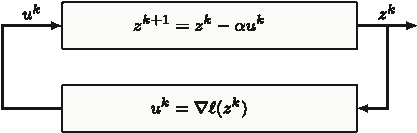
\includegraphics[width=0.55\linewidth]{./img/_gradient_method_integrator.pdf}
        \end{figure}
\end{description} 

\begin{theorem}[Gradient method convergence] \marginnote{Gradient method convergence}
    Consider a function $l$ such that:
    \begin{itemize}
        \item $\nabla l$ is $L$-Lipschitz continuous,
        \item The step size is constant or diminishing. 
    \end{itemize}
    Let $\{ \z^k \}_{k \in \mathbb{N}}$ be the (bounded) sequence generated by the gradient method. It holds that every limit point $\bar{\z}$ of the sequence $\{ \z^k \}_{k \in \mathbb{N}}$ is a stationary point (i.e., $\nabla l(\bar{z}) = 0$).

    In addition, if $l$ is $\mu$-strongly convex and the step size is constant, then the convergence rate of the sequence $\{ \z^k \}_{k \in \mathbb{N}}$ is exponential (also said geometric or linear):
    \[
        \Vert \z^k - \z^* \Vert \leq M \rho^k
    \]
    where $\rho \in (0, 1)$ and $M > 0$ depends on $\mu$, $L$, and $\Vert \z^0 - \z^* \Vert$.

    \begin{proof}
        We need to prove the two parts of the theorem:
        \begin{enumerate}
            \item 
                We want to prove that any limit point of the sequence generated by the gradient method is a stationary point.

                In other words, by considering the gradient method as an integrator with feedback, we want to analyze the equilibrium of the system. Assume that the system converges to some equilibrium $\z_E$. To be an equilibrium, it must be that the feedback loop stopped updating the system (i.e., $\vec{u}^k = 0$ for $k$ after some threshold) so that:
                \[
                    \z_E = \z_E - \alpha \nabla l(\z_E)
                \]
                Therefore, an equilibrium point is necessarily a stationary point of $l$ as it must be that $\nabla l(\z_E) = 0$.
            
            \item 
                We want to prove that if $l$ is $\mu$-strongly convex and the step size is constant, the sequence converges exponentially.

                \begin{remark}
                    As $l$ is convex, its equilibrium is also the global minimum $\z^*$.
                \end{remark}

                Consider the following change in coordinates (i.e., a translation):
                \[ 
                    \begin{gathered}
                        \z^k \mapsto \tilde{\z}^k \\
                        \text{with } \tilde{\z}^k = \z^k - \z_E = \z^k - \z^*
                    \end{gathered}
                \]
                The system in the new coordinates becomes:
                \[
                    \begin{aligned}
                        &\tilde{\z}^{k+1} = \tilde{\z}^k - \alpha \vec{u}^k \\
                        &\begin{aligned}
                            \vec{u}^k &= \nabla l(\z^k) \\
                            &= \nabla l(\tilde{\z}^k + \z^*) \\
                            &= \nabla l(\tilde{\z}^k + \z^*) - \nabla l(\z^*) & & & \text{\small $\nabla l(\z^*)=0$, but useful for \Cref{th:strong_convex_lipschitz_gradient}}
                        \end{aligned}
                    \end{aligned}
                \]

                \begin{figure}[H]
                    \centering
                    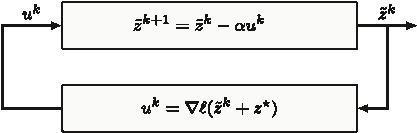
\includegraphics[width=0.55\linewidth]{./img/_gradient_method_integrator_new_coords.pdf}
                \end{figure}

                \begin{remark}
                    As $l$ is strongly convex and its gradient Lipschitz continuous, by \Cref{th:strong_convex_lipschitz_gradient} it holds that:
                    \[
                        -(\vec{u}^k)^T \tilde{\z}^k \leq - \gamma_1 \Vert \tilde{\z}^k \Vert^2 - \gamma_2 \Vert \tilde{\vec{u}}^k \Vert^2
                    \]
                \end{remark}

                Consider a Lyapunov function $V: \mathbb{R}^d \rightarrow \mathbb{R}_{\geq 0}$ defined as:
                \[
                    V(\tilde{\z}) = \Vert \tilde{\z} \Vert^2
                \]
                It holds that:
                \[
                    \begin{aligned}
                        V(\tilde{\z}^{k+1}) - V(\tilde{\z}^k) &= \Vert \tilde{\z}^{k+1} \Vert^2 - \Vert \tilde{\z}^k \Vert^2 \\
                        &= \Vert \tilde{\z}^{k} - \alpha \vec{u}^{k} \Vert^2 - \Vert \tilde{\z}^k \Vert^2 \\
                        &= \cancel{\Vert \tilde{\z}^k \Vert^2} - 2\alpha(\vec{u}^k)^T\tilde{\z}^k + \alpha^2 \Vert \vec{u}^k \Vert^2 - \cancel{\Vert \tilde{\z}^k \Vert^2} \\
                        &\leq -2\alpha\gamma_1 \Vert\tilde{\z}^k\Vert^2 + \alpha(\alpha-2\gamma_2) \Vert\vec{u}^k\Vert^2 &&& \text{\Cref{th:strong_convex_lipschitz_gradient}} 
                    \end{aligned}
                \]

                By choosing $\alpha \leq 2\gamma_2$, we have that:
                \[
                    \begin{split}
                        V(\tilde{\z}^{k+1}) - V(\tilde{\z}^k) &\leq -2\alpha\gamma_1 \Vert \tilde{\z}^k \Vert^2 \\
                        \iff \Vert \tilde{\z}^{k+1} \Vert^2 - \Vert \tilde{\z}^k \Vert^2 &\leq -2\alpha\gamma_1 \Vert \tilde{\z}^k \Vert^2 \\
                        \iff \Vert \tilde{\z}^{k+1} \Vert^2 &\leq (1-2\alpha\gamma_1) \Vert \tilde{\z}^k \Vert^2 \\
                    \end{split}
                \]
                Finally, as the gradient method is an iterative descent algorithm, it holds that:
                \[
                    \begin{split}
                        \Vert \tilde{\z}^{k+1} \Vert^2 &\leq (1-2\alpha\gamma_1) \Vert \tilde{\z}^k \Vert^2 \\
                        &\leq \dots \\
                        &\leq (1-2\alpha\gamma_1)^k \Vert \tilde{\z}^0 \Vert^2 \\
                    \end{split}
                \]
                Therefore, the sequence $\{ \tilde{\z}^k \}_{k \in \mathbb{R}}$ goes exponentially fast to zero and we have shown that:
                \[
                    \begin{split}
                        \Vert \z^{k+1} - \z^* \Vert^2 &\leq (1-2\alpha\gamma_1)^k \Vert \z^0 - \z^* \Vert^2 \\
                        &= \rho^k M
                    \end{split}
                \]
        \end{enumerate}
    \end{proof}
\end{theorem}

\begin{remark}[Gradient method for a quadratic function] \marginnote{Gradient method for a quadratic function}
    Given the problem of minimizing a quadratic function:
    \[
        \min_{\z} \frac{1}{2}\z^T \matr{Q} \z + \vec{r}^T \z
        \qquad
        \nabla l = \matr{Q} \z + \vec{r}
    \]
    The gradient method can be reduced to an affine linear system:
    \[
        \begin{split}
            \z^{k+1} &= \z^k - \alpha (\matr{Q} \z^k + \vec{r}) \\
            &= (\matr{I} - \alpha \matr{Q}) \z^k - \alpha \vec{r}
        \end{split}
    \]
    For a sufficiently small $\alpha$, the matrix $(\matr{I} - \alpha \matr{Q})$ is Schur (i.e., $\forall \matr{\rho}, |\matr{\rho}| < 1: \sum_{i=0}^{\infty} \matr{\rho}^i = (1-\matr{\rho})^{-1}$). Therefore, the solution can be computed in closed form as:
    \[
        \begin{split}
            \z^k &= (\matr{I} - \alpha \matr{Q})^k \z^0 - \alpha \sum_{\tau=0}^{k-1} (\matr{I} - \alpha \matr{Q})^\tau \vec{r} \\
            &\overset{k \rightarrow \infty}{\longrightarrow} - \alpha \left( \sum_{\tau=0}^{\infty} (\matr{I} - \alpha \matr{Q})^\tau \right) \vec{r} = -\matr{Q}^{-1} \vec{r}
        \end{split}
    \]
\end{remark}

\begin{remark}[Gradient flow] \marginnote{Gradient flow}
    By inverting the integrator and plant of the discrete-time integrator of the gradient method, and considering the continuous-time case, the result is the gradient flow:
    \[
        \dot{\z}(t) = -\nabla l(\z(t))
    \]
    which has a solution if the vector field is Lipschitz continuous.

    \begin{figure}[H]
        \centering
        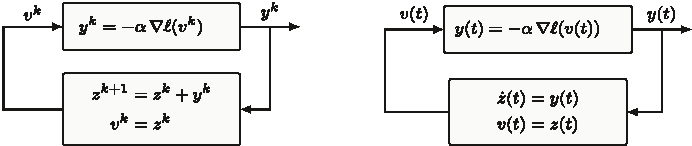
\includegraphics[width=0.8\linewidth]{./img/_gradient_flow.pdf}
    \end{figure}
\end{remark}


\subsection{Accelerated gradient methods}

\begin{description}
    \item[Heavy-ball method] \marginnote{Heavy-ball method}
        Given $\eta^0$ and $\eta^{-1}$, the algorithm is defined as:
        \[
            \eta^{k+1} = \eta^k + \alpha_1 (\eta^k - \eta^{k-1}) - \alpha_2 \nabla l(\eta^k)
        \]
        with $\alpha_1, \alpha_2 > 0$.

        \begin{remark}
            With $\alpha_1 = 0$, the algorithm is reduced to the gradient method with step size $\alpha_2$.
        \end{remark}

        \begin{remark}
            The algorithm admits a state-space representation as a discrete-time integrator with a feedback loop:
            \begin{figure}[H]
                \centering
                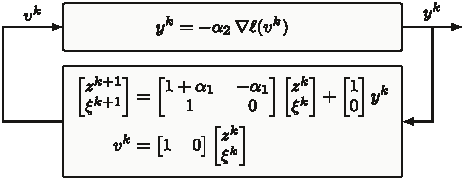
\includegraphics[width=0.55\linewidth]{./img/_heavy_ball.pdf}
            \end{figure}

            Note that the matrix $\begin{bmatrix} 1+\alpha_1 & -\alpha_1 \\ 1 & 0 \end{bmatrix}$ is row stochastic.
        \end{remark}

    \item[Generalized heavy-ball method] \marginnote{Generalized heavy-ball method}
        Given $\zeta^0$ and $\zeta^{-1}$, the algorithm is defined as:
        \[
            \zeta^{k+1} = \zeta^k + \alpha_1 (\zeta^k - \zeta^{k-1}) - \alpha_2 \nabla l(\zeta^k + \alpha_3(\zeta^k - \zeta^{k-1}))
        \]
        with $\alpha_1, \alpha_2, \alpha_3 > 0$.

        \begin{remark}
            The algorithm admits a state-space representation as a discrete-time integrator with a feedback loop:
            \begin{figure}[H]
                \centering
                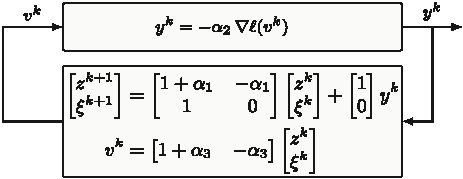
\includegraphics[width=0.55\linewidth]{./img/_generalized_heavy_ball.pdf}
            \end{figure}
        \end{remark}
\end{description}



\section{Cost-coupled optimization}


\begin{description}
    \item[Cost-coupled optimization] \marginnote{Cost-coupled optimization}
        Problem of minimizing $N$ cost functions $l_i: \mathbb{R}^d \rightarrow \mathbb{R}$, each local and private to an agent:
        \[
            \min_{\z \in \mathbb{R}^{d}} \sum_{i=1}^{N} l_i(\z)
        \]
\end{description}


\subsection{Learning paradigms}

\begin{description}
    \item[Federated learning] \marginnote{Federated learning}
        Problem where $N$ agents with their local and private data $\mathcal{D}^{i}$ want to learn a common set of parameters $\z^*$ based on the same loss function (evaluated on different data points):
        \[
            \min_\z \sum_{i=1}^{N} l(\z; \mathcal{D}^i)
        \]
        A centralized parameter server (master) is responsible for aggregating the estimates of the agents (e.g., pick some nodes and average them).
        % \[
        %     \z^{t+1} = \z^k - \alpha \sum_{i \in I_k} \nabla l(\z; \mathcal{D}^i, p^i)
        % \]

    \item[Distributed learning] \marginnote{Distributed learning}
        Federated learning where there is no centralized entity and agents communicate with their neighbors only.
\end{description}

\begin{figure}[H]
    \centering
    \begin{subfigure}{0.4\linewidth}
        \centering
        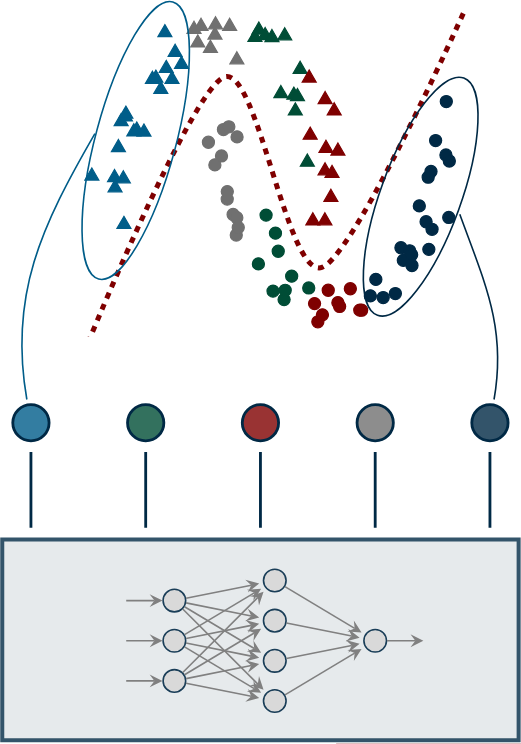
\includegraphics[width=0.55\linewidth]{./img/federated_learning.png}
        \caption{Federated learning}
    \end{subfigure}
    \begin{subfigure}{0.4\linewidth}
        \centering
        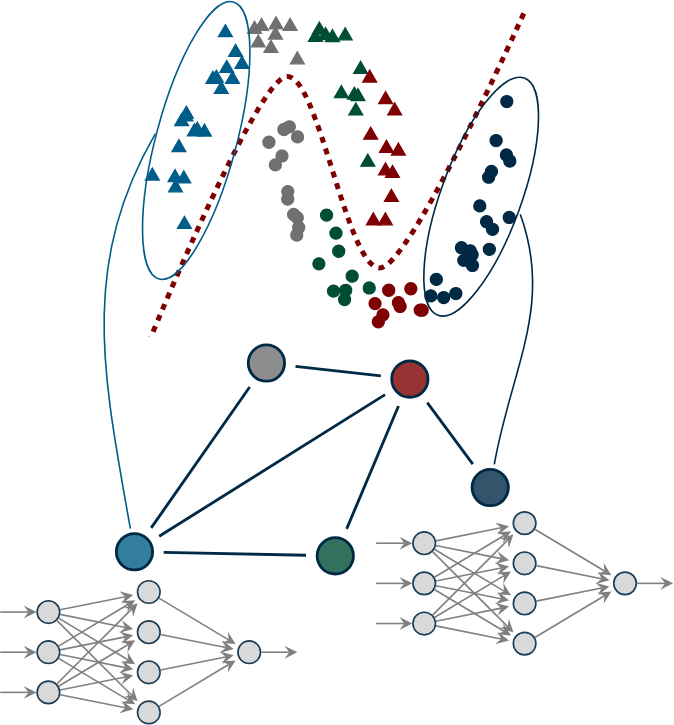
\includegraphics[width=0.7\linewidth]{./img/distributed_learning.png}
        \caption{Distributed learning}
    \end{subfigure}
\end{figure}



\section{Federated learning}


\subsection{Batch gradient method}

\begin{description}
    \item[Batch gradient method] \marginnote{Batch gradient method}
        Compute the direction for the gradient method by considering all the losses:
        \[
            \z^{k+1} = \z^k - \alpha \sum_{i=1}^{N} \nabla l_i(\z^k)
        \]

        \begin{remark}
            Computation in this way can be expensive.
        \end{remark}
\end{description}


\subsection{Incremental gradient method}

\begin{description}
    \item[Incremental gradient method] \marginnote{Incremental gradient method}
        At each iteration $k$, compute the direction by considering the loss of a single agent $i^k$:
        \[
            \z^{k+1} = \z^k - \alpha \nabla l_{i^k}(\z^k)
        \]

        \begin{remark}
            Two possible rules to select the agent at each iteration are:
            \begin{descriptionlist}
                \item[Cyclic] 
                    $i^k = 1, 2, \dots, N, 1, 2, \dots, N, \dots$, or cyclic in any order (essentially cyclic).
                \item[Randomized] 
                    Draw $i^k$ from a uniform distribution.
            \end{descriptionlist}
        \end{remark}

        \begin{remark}
            A single gradient is not necessarily a descent direction.
        \end{remark}

        \begin{theorem}
            If the step size is diminishing, the incremental gradient method converges.
        \end{theorem}
\end{description}


\subsection{Stochastic gradient descent}

\begin{description}
    \item[Stochastic gradient descent (SGD)] \marginnote{Stochastic gradient descent (SGD)}
        Instance of incremental gradient method where the selection rule follows an unknown distribution.

        The problem can be formulated as:
        \[ \min_{\z \in \mathbb{R}^d} \mathbb{E}_\mathcal{W}[l(\z, \mathcal{W})] \]
        where $\mathcal{W}$ is a random variable with possibly an unknown distribution.

        It is assumed that, given any realization $\bar{w}$ of $\mathcal{W}$ (e.g., the index of an agent or a single data point), it is possible to obtain the gradient $\nabla l(\bar{\z}, \bar{w})$ at any query point $\bar{\z}$. The optimization step at each iteration is then:
        \[ \z^{k+1} = \z^k - \alpha \nabla l(\z^k, w^k) \]
        
        \begin{remark}
            Monte Carlo approximation can be used to represent the expected value with a finite sequence of realizations:
            \[ \mathbb{E}_\mathcal{W}[l(\z, \mathcal{W})] \approx \frac{1}{K} \sum_{k=1}^{K} l(\z, w^k) \]
        \end{remark}

        \begin{theorem}[SGD convergence with constant step size] \marginnote{SGD convergence with constant step size}
            Given a function $l$ such that:
            \begin{itemize}
                \item $l$ is $\mu$-strongly convex with $L$-Lipschitz continuous gradient (i.e., bounded),
                \item $\nabla l(\z, \mathcal{W})$ is an unbiased estimate of $\nabla_\z \mathbb{E}_\mathcal{W}[l(\z, \mathcal{W})]$,
                \item $\Vert \nabla l(\z, \mathcal{W}) \Vert \leq M_\nabla$ almost surely (i.e., asymptotically with probability $1$) for some $M_\nabla > 0$.
            \end{itemize}
            With a constant step size $\alpha \leq \frac{1}{2}\mu$, it holds that at any time step $k$:
            \[ 
                \Vert \z^k - \z^* \Vert \leq 
                \underbrace{(1-2\mu\alpha)^k \left( \Vert \z^0 - \z^* \Vert - \frac{\alpha M_\nabla^2}{2\mu} \right)}_{\text{Error term}} + 
                \underbrace{\frac{\alpha M_\nabla^2}{2\mu}}_{\text{Residual term}} \]
            where the error diminishes over time and the residual term is constant.
        \end{theorem}

        \begin{theorem}[SGD convergence with diminishing step size] \marginnote{SGD convergence with diminishing step size}
            With a diminishing step size, both the error and the residual converge to $0$.
        \end{theorem}

    \item[Mini-batch SGD] \marginnote{Mini-batch SGD}
        SGD where the update at each time step $k$ is based on a set $\mathcal{I}^k \subset \{ 1, \dots, N \}$ of realizations of $\mathcal{W}$:
        \[ \z^{k+1} = \z^k - \alpha \sum_{i \in \mathcal{I}^k} \nabla l(\z^k, w^i) \]
\end{description}


\subsection{Adaptive momentum}

\begin{description}
    \item[Adaptive momentum (ADAM)] \marginnote{Adaptive momentum (ADAM)}
        Method based on the first and second momentum of the gradient:
        \[
            \begin{split}
                \vec{m}^{k+1} &= \beta_1 \vec{m}^k + (1-\beta_1) \nabla l(\z^k, w^k) \\
                \vec{v}^{k+1} &= \beta_2 \vec{v}^k + (1-\beta_2) \left( \nabla l(\z^k, w^k) \right)^2
            \end{split}
        \]
        where $\beta_1, \beta_2 \in (0, 1)$ are hyperparameters.
        
        The descent direction is defined as:
        \[
            \begin{gathered}
                \hat{\vec{m}} = \frac{1}{1 - \beta_1^{k+1}} \vec{m}^{k+1}
                \quad
                \hat{\vec{v}} = \frac{1}{1 - \beta_2^{k+1}} \vec{v}^{k+1} \\
                \vec{d}^k = - \frac{\hat{\vec{m}}}{\sqrt{\hat{\vec{v}}} + \varepsilon} \\
            \end{gathered}
        \]
        The update is performed as:
        \[ \z^{k+1} = \z^{k} + \alpha \vec{d}^k \]
\end{description}



\section{Distributed cost-coupled/consensus optimization}

\begin{description}
    \item[Distributed cost-coupled optimization] \marginnote{Distributed cost-coupled optimization}
        Optimization problem with $N$ agents that communicate according to a graph $G$ aiming at learning a common set of parameters $\z$ such that:
        \[
            \min_{\z \in Z} \sum_{i=1}^{N} l_i(\z)
        \]
        where:
        \begin{itemize}
            \item Each agent $i$ knows its loss $l_i$ (based on its available data) and the parameter space $Z$,
            \item At each time step $k$, each agent $i$ estimates a set of parameters $\z_i^k$.
        \end{itemize}

        \begin{figure}[H]
            \centering
            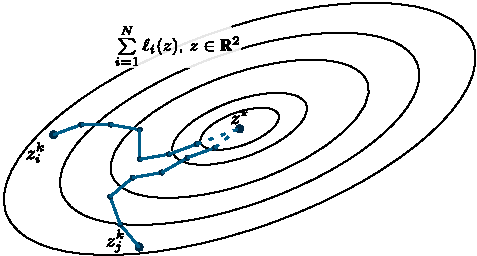
\includegraphics[width=0.45\linewidth]{./img/_distributed_cost_coupled.pdf}
        \end{figure}
\end{description}

\begin{remark}
    Using as direction the sum of the gradients of all agents is not possible as not everyone can communicate with everyone.
\end{remark}


\subsection{Distributed gradient algorithm}

\begin{description}
    \item[Distributed gradient algorithm] \marginnote{Distributed gradient algorithm}
        Method that estimates a (more precise) set of parameters as a weighted sum those of its neighbors' (self-loop included):
        \[ 
            \vec{v}_i^{k+1} = \sum_{j \in \mathcal{N}_i} a_{ij} \z_j^k 
        \]
        Then, the update step is performed using $\vec{v}_i^{k+1}$ and the agent's own local loss $l_i$:
        \[
            \begin{split}
                \z_i^{k+1} &= \vec{v}_i^{k+1} - \alpha^k \nabla l_i(\vec{v}_i^{k+1}) \\
                &= \left(\sum_{j \in \mathcal{N}_i} a_{ij} \z_j^k\right) - \alpha^k \nabla l_i\left(\sum_{j \in \mathcal{N}_i} a_{ij} \z_j^k\right)
            \end{split}
        \]
\end{description}

\begin{theorem}[Distributed gradient algorithm convergence] \marginnote{Distributed gradient algorithm convergence}
    Assume that:
    \begin{itemize}
        \item The matrix $\matr{A}$ associated to the undirected and connected communication graph $G$ is doubly stochastic and such that $a_{ij} > 0$,
        \item The step size is diminishing,
        \item Each $l_i$ is convex, has gradients bounded by a scalar $C_i > 0$, and there exists at least one optimal solution.
    \end{itemize}
    Then, the sequence of local solutions $\{ \z_i^k \}_{k \in \mathbb{N}}$ of each agent $i$ produced using the distributed gradient algorithm converges to a common optimal solution $\z^*$:
    \[ \lim_{k \rightarrow \infty} \Vert \z_i^k - \z^* \Vert = 0 \]
\end{theorem}


\begin{description}
    \item[Distributed projected subgradient algorithm] \marginnote{Distributed projected subgradient algorithm}
        Distributed gradient algorithm extended to the case where $l_i$ are non-smooth convex functions and $\z$ is constrained to a closed convex set $Z \subseteq \mathbb{R}^d$. The distributed step is the following:
        \[
            \begin{split}
                \vec{v}_i^{k+1} &= \sum_{j \in \mathcal{N}_i} a_{ij} \z_j^k \\
                \z_i^{k+1} &= P_Z \big( \vec{v}_i^{k+1} - \alpha^k \tilde{\nabla} l_i(\vec{v}_i^{k+1}) \big)
            \end{split}
        \]
        where $P_Z(\cdot)$ is the Euclidean projection onto $Z$ and $\tilde{\nabla} l_i$ is a subgradient of $l_i$.
\end{description}

\begin{theorem}[Distributed projected subgradient algorithm convergence] \marginnote{Distributed projected subgradient algorithm convergence}
    Assume that:
    \begin{itemize}
        \item The adjacency matrix $\matr{A}$ associated to $G$ is doubly stochastic and $a_{ij} > 0$,
        \item The step size is diminishing,
        \item Each $l_i$ is convex, has subgradients bounded by a scalar $C_i > 0$, and there exists at least one optimal solution.
    \end{itemize}
    Then, each agent converges to an optimal solution $\z^*$.
\end{theorem}

\begin{theorem}
    The distributed gradient algorithm does not converge with a constant step size.

    \begin{proof}[Proof idea]
        % Assume that the starting guess in standard gradient descent is is a local minimum:
        % \[ \z^{0} = \z^* \]
        % We have that:
        % \[
        %     \begin{split}
        %         \z^* &= \z^* - \alpha \nabla l(\z^*) \\
        %         \z^* &= \z^* \\
        %     \end{split}
        % \]
        % $\z^*$ is an equilibrium.

        We want to check whether the optimum $\z^*$ with a constant step size $\alpha$ is an equilibrium:
        \[
            \begin{aligned}
                \z^* &= \sum_{j=1}^N a_{ij} \z^* - \alpha \nabla l_i \left( \sum_{j=1}^N a_{ij} \z^* \right) \\
                &= \z^* - \alpha \nabla l_i (\z^*) &&& \parbox{0.20\linewidth}{\footnotesize $\matr{A}$ doubly stochastic and $\z^*$ constant} \\
            \end{aligned}
        \]
        In general, $\nabla l_i(\z^*) \neq 0$ ($\z^*$ is the optimum for the whole problem, but $l_i$ depends on the subset of data available to the agent). Therefore, $\z^*$ is not an equilibrium.
    \end{proof}
\end{theorem}


\subsection{Gradient tracking algorithm} \label{sec:gradient_tracking_algorithm}

\begin{description}
    \item[Dynamic average consensus] \marginnote{Dynamic average consensus}
        Consensus algorithm where each agent measures a signal $r_i^k$ and wants to estimate the average signal of all agents:
        \[ \bar{r}^k = \frac{1}{N} \sum_{i=1}^{N} r_i^k \]
        The average signal estimated by an agent is represented by a state $s_i^k$ and we want that $\lim_{k \rightarrow \infty} \Vert s_i^k - \bar{r}^k \Vert = 0$. This can be achieved using a perturbed consensus algorithm:
        \[ 
            s_i^{k+1} = 
            \underbrace{\sum_{j \in \mathcal{N}_i} a_{ij} s_j^k}_{\text{Consensus}} +
            \underbrace{\vphantom{\sum_{j \in \mathcal{N}_i}}(r_i^{k+1} - r_i^k)}_{\text{Innovation}}
        \]
        where:
        \begin{itemize}
            \item The consensus term converges to the states average.
            \item The local innovation allows converging to the common signal.
        \end{itemize}

        \begin{theorem}[Dynamic average consensus convergence]
            If the first-order differences are bounded (i.e., $\Vert r_i^{k+1} - r_i^{k} \Vert \leq C_1$), then the tracking error is bounded by some $C_2 > 0$:
            \[ \lim_{k \rightarrow \infty} \Vert s_i^k - \bar{r}^k \Vert \leq C_2 \]

            Moreover, the error is zeroed if the signal becomes constant after some time $k$ (i.e., $\Vert r_i^{k+1} - r_i^{k} \Vert \rightarrow 0$).
        \end{theorem}

    \item[Gradient tracking algorithm] \marginnote{Gradient tracking algorithm}
        Method that chooses the local descent direction attempting to asymptotically track the true gradient:
        \[ d_i^k \underset{k \rightarrow \infty}{\longrightarrow} - \frac{1}{N} \sum_{h=1}^N \nabla l_h(\z_h^k) \] 

        By using dynamic average consensus, we consider as signal the local gradient:
        \[ \vec{r}_i^k = \nabla l_i(\z_i^k) \]
        Then, the estimate of the average signal (i.e., gradient) is given by:
        \[
            \vec{s}_i^{k+1} = \sum_{j \in \mathcal{N}_i} a_{ij} \vec{s}_j^k + \left( \nabla l_i(\z_i^{k+1}) - \nabla l_i(\z_i^k) \right) \qquad \s_i^0 = \nabla l_i(\z_i^0)
        \]
        The update step is then performed as:
        \[ \z_i^{k+1} = \sum_{j \in \mathcal{N}_i} a_{ij} \z_j^k - \alpha \vec{s}_i^k \]

        % Each agent accesses some $\nabla l_i(\z)$. It can be seen as a signal $r_i^k = \nabla l_i(\z_i^k)$ only available at agent $i$.

        % We want that the direction:
        % \[ d_i^k \underset{k \rightarrow \infty}{\longrightarrow} - \frac{1}{N} \sum_{h=1}^N r_h^k \] 

        % Ideally, we want:
        % \[
        %     \z_i^{k+1} = \sum_{j=1}^N a_{ij} \z_j^k - (N\alpha) \frac{1}{N} \sum_{j=1}^N \nabla l_k(z_k^k)
        % \]

        \begin{theorem}[Gradient tracking algorithm optimality] \marginnote{Gradient tracking algorithm optimality}
            If:
            \begin{itemize}
                \item $\matr{A}$ is the adjacency matrix of an undirected and connected communication graph $G$ such that it is doubly stochastic and $a_{ij} > 0$.
                \item Each cost function $l_i$ is $\mu$-strongly convex and its gradient $L$-Lipschitz continuous.
            \end{itemize}
            Then, there exists $\alpha^* > 0$ such that, for any choice of the step size $\alpha \in (0, \alpha^*)$, the sequence of local solutions $\{ \z_i^k \}_{k \in \mathbb{N}}$ of each agent generated by the gradient tracking algorithm asymptotically converges to a consensual optimal solution $\z^*$:
            \[ \lim_{k \rightarrow \infty} \Vert \z_i^k - \z^* \Vert = 0 \]
            
            Moreover, the convergence rate is linear and stability is exponential:
            \[ 
                \exists \rho \in (0,1): \Vert \z_i^k - \z^* \Vert \leq \rho \Vert \z_i^{k+1} - \z^* \Vert
                \,\,\land\,\,
                \rho \Vert \z_i^{k+1} - \z^* \Vert \leq \rho^k \Vert \z_i^0 - \z^* \Vert
            \]

            {
                \indenttbox
                \begin{remark}
                    It can be shown that gradient tracking also works with non-convex optimization and, under the correct assumptions, converges to a stationary point. 
                \end{remark}
            }

            \begin{proof}
                Consider the gradient tracking algorithm written in matrix form:
                \[
                    \begin{aligned}
                        \z^{k+1} &= \A \z^k - \alpha \s^k \\
                        \s^{k+1} &= \A \s^k + (\nabla \vec{l}(\z^{k+1}) - \nabla \vec{l}(\z^k))
                    \end{aligned}
                \]
                where $\nabla \vec{l}(\z^k) = \begin{bmatrix} l_1(\z^k_1) & \dots & l_N(\z^k_N) \end{bmatrix}$.

                % \begin{remark}
                %     In the vector case, the Kronecker product should be applied on $\A$.
                % \end{remark}

                \begin{description}
                    \item[Equilibrium]
                        We want to find the equilibrium points $(\z_\text{eq}, \s_\text{eq})$ that satisfies:
                        \[
                            \begin{aligned}
                                \s_\text{eq} &= \A \s_\text{eq} + \nabla \vec{l}(\z_\text{eq}) - \nabla \vec{l}(\z_\text{eq}) &\iff& (\matr{I} - \A) \s_\text{eq} = 0 \\
                                \z_\text{eq} &= \A\z_\text{eq} - \alpha \s_\text{eq} &\iff& (\matr{I} - \A) \z_\text{eq} = -\alpha \s_\text{eq} \\
                            \end{aligned}
                        \]
                        It must be that:
                        \begin{itemize}
                            \item $\s_\text{eq} \in \text{ker}(\matr{I} - \A) = \{ \vec{1}\beta_1 \mid \beta_1 \in \R \}$ (as $\A$ is doubly stochastic).
                            \item $(\matr{I} - \A) \z_\text{eq} = - \alpha \vec{1} \beta_1$. As $\vec{1} (-\alpha \beta_1) \in \text{ker}(\matr{I} - \A)$, it must be that $\beta_1 = 0$ (as the image cannot be mapped into the kernel).
                        \end{itemize}
                        Therefore, we end up with:
                        \[
                            \begin{split}
                                \s_\text{eq} &= \vec{1}\beta_1 = 0 \\
                                \z_\text{eq} &= \A\z_\text{eq} - \alpha 0 = \matr{1} \beta_2 \quad \text{ i.e., eigenvector of $\A$} \\
                            \end{split}
                        \]

                        In addition, by pre-multiplying the equation of $\s$ by $\vec{1}^T$, we obtain:
                        \[
                            \begin{split}
                                \vec{1}^T \s^{k+1} &= \vec{1}^T \A \s^k + \vec{1}^T \nabla \vec{l}(\z^{k+1}) - \vec{1}^T \nabla \vec{l}(\z^{k}) \\
                                &= \vec{1}^T \s^k + \vec{1}^T \nabla \vec{l}(\z^{k+1}) - \vec{1}^T \nabla \vec{l}(\z^{k}) 
                            \end{split}
                        \]
                        Which shows the following invariance condition:
                        \[ 
                            \begin{aligned}
                                \vec{1}^T \s^{k+1} - \vec{1}^T \nabla \vec{l}(\z^{k+1})
                                &= \vec{1}^T \s^k - \vec{1}^T \nabla \vec{l}(\z^{k}) \\
                                &= \vec{1}^T \s_\text{eq} - \vec{1}^T \nabla \vec{l}(\z_\text{eq}) \\
                                &= \vec{1}^T \s^0 - \vec{1}^T \nabla \vec{l}(\z^{0}) \\
                            \end{aligned}
                        \]
                        Thus, we have that:
                        \[
                            \begin{split}
                                \vec{1}^T \s_\text{eq} - \vec{1}^T \nabla \vec{l}(\z_\text{eq})
                                &= \vec{1}^T \s^0 - \vec{1}^T \nabla \vec{l}(\z^{0}) \\
                                \iff 0 - \vec{1}^T \nabla \vec{l}(\vec{1}\beta_2) &= 0 \\
                            \end{split}
                        \]
                        Then, it must be that $\z_\text{eq} = \vec{1}\beta_2$ is an optimum with $\beta_2 = z^*$.
                
                    \item[Stability]
                        % Change in coordinates to avoid having $\z^{k+1}$ in $\s^{k}$. The (non-linear) transformation is:
                        % \[
                        %     \begin{bmatrix}
                        %         \z^k \\ \s^k
                        %     \end{bmatrix}
                        %     \mapsto
                        %     \begin{bmatrix}
                        %         \z^k \\ \vec{\xi}^k
                        %     \end{bmatrix}
                        %     =
                        %     \begin{bmatrix}
                        %         \z^k \\ \alpha (\nabla \vec{l}(\z^k) - \s^k)
                        %     \end{bmatrix}
                        % \]

                        % \[
                        %     \begin{split}
                        %         \z^{k+1} 
                        %         &= \A\z^k - \alpha ( \frac{1}{\alpha} \vec{\xi}^k + \nabla \vec{l}(\z^k) ) \\
                        %         \vec{\xi}^k 
                        %         &= \alpha \nabla \vec{l}(\z^{k+1}) - \alpha (\A \s^k + \nabla \vec{l}(\z^{k+1}) - \nabla \vec{l} (\z^k)) \\
                        %         &= - \alpha \A (-\frac{1}{\alpha} \xi^k + \nabla \vec{l}(\z^k)) + \alpha \nabla \vec{l}(\z^k) \\
                        %         &= \A \vec{\xi}^k - \alpha(\A - \vec{I}) \nabla \vec{l}(\z^k)
                        %     \end{split}
                        % \]

                        % In matrix form:
                        % \[
                        %     \begin{bmatrix}
                        %         \z^{k+1} \\ \vec{\xi}^{k+1} = \begin{bmatrix}
                        %             \A & \matr{I} \\ 0 & \A
                        %         \end{bmatrix}
                        %         \begin{bmatrix}
                        %             \z^k \\ \vec{\xi}^k
                        %         \end{bmatrix}
                        %         - alpha \begin{bmatrix}
                        %             \matr{I} \\ \A \matr{I}
                        %         \end{bmatrix}
                        %         \nabla \vec{l}(\z^k)
                        %     \end{bmatrix}
                        % \]
                        % The initialization is:
                        % \[
                        %     \begin{split}
                        %         \z^0 \in \R^N \\
                        %         \vec{\xi}^{0} = \alpha (\nabla \vec{l}(\z^0) - \s^0) = 0
                        %     \end{split}
                        % \]
                        % The equilibrium has been shifted to:
                        % \[
                        %     \begin{split}
                        %         \z_\text{eq} = \vec{1} \z^* \\
                        %         \vec{\xi}_\text{eq} = \alpha \nabla l(\vec{1} \z^*) = \alpha \begin{bmatrix}
                        %             \nabla l_1(\z^*) \\ \vdots \\ \nabla l_N(\z^*)
                        %         \end{bmatrix}
                        %     \end{split}
                        % \]


                        % \[
                        %     \begin{gathered}
                        %         \begin{bmatrix}
                        %             \z^{k+1} \\ \vec{\xi}^{k+1} = \begin{bmatrix}
                        %                 \A & \matr{I} \\ 0 & \A
                        %             \end{bmatrix}
                        %             \begin{bmatrix}
                        %                 \z^k \\ \vec{\xi}^k
                        %             \end{bmatrix}
                        %             \begin{bmatrix}
                        %                 \matr{I} \\ \A \matr{I}
                        %             \end{bmatrix}
                        %             \u^k
                        %         \end{bmatrix} \\
                        %         \vec{y}^k = \begin{bmatrix}
                        %             \matr{I} & 0
                        %         \end{bmatrix}
                        %         \begin{bmatrix}
                        %             \z^k \\ \vec{\xi}^{k}
                        %         \end{bmatrix} \\
                        %         -- \\
                        %         \u^k = \nabla \vec{l}(\vec{y}^k)
                        %     \end{gathered}
                        % \]
                \end{description}
            \end{proof}
        \end{theorem}
\end{description}
